\documentclass[]{article}
\usepackage{lmodern}
\usepackage{amssymb,amsmath}
\usepackage{ifxetex,ifluatex}
\usepackage{fixltx2e} % provides \textsubscript
\ifnum 0\ifxetex 1\fi\ifluatex 1\fi=0 % if pdftex
  \usepackage[T1]{fontenc}
  \usepackage[utf8]{inputenc}
\else % if luatex or xelatex
  \ifxetex
    \usepackage{mathspec}
  \else
    \usepackage{fontspec}
  \fi
  \defaultfontfeatures{Ligatures=TeX,Scale=MatchLowercase}
\fi
% use upquote if available, for straight quotes in verbatim environments
\IfFileExists{upquote.sty}{\usepackage{upquote}}{}
% use microtype if available
\IfFileExists{microtype.sty}{%
\usepackage{microtype}
\UseMicrotypeSet[protrusion]{basicmath} % disable protrusion for tt fonts
}{}
\usepackage[margin=1in]{geometry}
\usepackage{hyperref}
\hypersetup{unicode=true,
            pdftitle={Atividade 3},
            pdfauthor={Guilherme Navarro NUSP: 8943160},
            pdfborder={0 0 0},
            breaklinks=true}
\urlstyle{same}  % don't use monospace font for urls
\usepackage{color}
\usepackage{fancyvrb}
\newcommand{\VerbBar}{|}
\newcommand{\VERB}{\Verb[commandchars=\\\{\}]}
\DefineVerbatimEnvironment{Highlighting}{Verbatim}{commandchars=\\\{\}}
% Add ',fontsize=\small' for more characters per line
\usepackage{framed}
\definecolor{shadecolor}{RGB}{248,248,248}
\newenvironment{Shaded}{\begin{snugshade}}{\end{snugshade}}
\newcommand{\KeywordTok}[1]{\textcolor[rgb]{0.13,0.29,0.53}{\textbf{#1}}}
\newcommand{\DataTypeTok}[1]{\textcolor[rgb]{0.13,0.29,0.53}{#1}}
\newcommand{\DecValTok}[1]{\textcolor[rgb]{0.00,0.00,0.81}{#1}}
\newcommand{\BaseNTok}[1]{\textcolor[rgb]{0.00,0.00,0.81}{#1}}
\newcommand{\FloatTok}[1]{\textcolor[rgb]{0.00,0.00,0.81}{#1}}
\newcommand{\ConstantTok}[1]{\textcolor[rgb]{0.00,0.00,0.00}{#1}}
\newcommand{\CharTok}[1]{\textcolor[rgb]{0.31,0.60,0.02}{#1}}
\newcommand{\SpecialCharTok}[1]{\textcolor[rgb]{0.00,0.00,0.00}{#1}}
\newcommand{\StringTok}[1]{\textcolor[rgb]{0.31,0.60,0.02}{#1}}
\newcommand{\VerbatimStringTok}[1]{\textcolor[rgb]{0.31,0.60,0.02}{#1}}
\newcommand{\SpecialStringTok}[1]{\textcolor[rgb]{0.31,0.60,0.02}{#1}}
\newcommand{\ImportTok}[1]{#1}
\newcommand{\CommentTok}[1]{\textcolor[rgb]{0.56,0.35,0.01}{\textit{#1}}}
\newcommand{\DocumentationTok}[1]{\textcolor[rgb]{0.56,0.35,0.01}{\textbf{\textit{#1}}}}
\newcommand{\AnnotationTok}[1]{\textcolor[rgb]{0.56,0.35,0.01}{\textbf{\textit{#1}}}}
\newcommand{\CommentVarTok}[1]{\textcolor[rgb]{0.56,0.35,0.01}{\textbf{\textit{#1}}}}
\newcommand{\OtherTok}[1]{\textcolor[rgb]{0.56,0.35,0.01}{#1}}
\newcommand{\FunctionTok}[1]{\textcolor[rgb]{0.00,0.00,0.00}{#1}}
\newcommand{\VariableTok}[1]{\textcolor[rgb]{0.00,0.00,0.00}{#1}}
\newcommand{\ControlFlowTok}[1]{\textcolor[rgb]{0.13,0.29,0.53}{\textbf{#1}}}
\newcommand{\OperatorTok}[1]{\textcolor[rgb]{0.81,0.36,0.00}{\textbf{#1}}}
\newcommand{\BuiltInTok}[1]{#1}
\newcommand{\ExtensionTok}[1]{#1}
\newcommand{\PreprocessorTok}[1]{\textcolor[rgb]{0.56,0.35,0.01}{\textit{#1}}}
\newcommand{\AttributeTok}[1]{\textcolor[rgb]{0.77,0.63,0.00}{#1}}
\newcommand{\RegionMarkerTok}[1]{#1}
\newcommand{\InformationTok}[1]{\textcolor[rgb]{0.56,0.35,0.01}{\textbf{\textit{#1}}}}
\newcommand{\WarningTok}[1]{\textcolor[rgb]{0.56,0.35,0.01}{\textbf{\textit{#1}}}}
\newcommand{\AlertTok}[1]{\textcolor[rgb]{0.94,0.16,0.16}{#1}}
\newcommand{\ErrorTok}[1]{\textcolor[rgb]{0.64,0.00,0.00}{\textbf{#1}}}
\newcommand{\NormalTok}[1]{#1}
\usepackage{longtable,booktabs}
\usepackage{graphicx,grffile}
\makeatletter
\def\maxwidth{\ifdim\Gin@nat@width>\linewidth\linewidth\else\Gin@nat@width\fi}
\def\maxheight{\ifdim\Gin@nat@height>\textheight\textheight\else\Gin@nat@height\fi}
\makeatother
% Scale images if necessary, so that they will not overflow the page
% margins by default, and it is still possible to overwrite the defaults
% using explicit options in \includegraphics[width, height, ...]{}
\setkeys{Gin}{width=\maxwidth,height=\maxheight,keepaspectratio}
\IfFileExists{parskip.sty}{%
\usepackage{parskip}
}{% else
\setlength{\parindent}{0pt}
\setlength{\parskip}{6pt plus 2pt minus 1pt}
}
\setlength{\emergencystretch}{3em}  % prevent overfull lines
\providecommand{\tightlist}{%
  \setlength{\itemsep}{0pt}\setlength{\parskip}{0pt}}
\setcounter{secnumdepth}{0}
% Redefines (sub)paragraphs to behave more like sections
\ifx\paragraph\undefined\else
\let\oldparagraph\paragraph
\renewcommand{\paragraph}[1]{\oldparagraph{#1}\mbox{}}
\fi
\ifx\subparagraph\undefined\else
\let\oldsubparagraph\subparagraph
\renewcommand{\subparagraph}[1]{\oldsubparagraph{#1}\mbox{}}
\fi

%%% Use protect on footnotes to avoid problems with footnotes in titles
\let\rmarkdownfootnote\footnote%
\def\footnote{\protect\rmarkdownfootnote}

%%% Change title format to be more compact
\usepackage{titling}

% Create subtitle command for use in maketitle
\providecommand{\subtitle}[1]{
  \posttitle{
    \begin{center}\large#1\end{center}
    }
}

\setlength{\droptitle}{-2em}

  \title{Atividade 3}
    \pretitle{\vspace{\droptitle}\centering\huge}
  \posttitle{\par}
    \author{Guilherme Navarro NUSP: 8943160}
    \preauthor{\centering\large\emph}
  \postauthor{\par}
      \predate{\centering\large\emph}
  \postdate{\par}
    \date{22 de junho de 2020}

\usepackage{multirow}
\usepackage{ragged2e}
\usepackage{booktabs}

\begin{document}
\maketitle

\section{Atividade 3}\label{atividade-3}

Um estudo foi conduzido em uma comunidade de Tartu, segunda maior cidade
da Estônia, para avaliar a sobrevida de pacientes que sofreram infarte
no período de 1991 a 1993 (com seguimento até 1996). Os dados
considerados são de 824 pacientes com 18 anos ou mais que tiveram
infarto no período de 1991 a 1993 e algumas variáveis foram observadas:

\begin{itemize}
\tightlist
\item
  Tempo de vida, em meses, após o infarto (os dados estão sujeitos a
  censura à direita);
\item
  Gênero (feminino ou masculino);
\item
  Idade (em anos);
\item
  Diagnóstico (Isquêmico/Hemorragia intracranial/Não
  identificado/hemorragia subaracnóide);
\item
  Coma - variável binária (Não/Sim) indicando se o paciente entrou em
  coma após o infarto;
\item
  Infarto prévio do miocárdio - variável binária (Não/Sim) indicando se
  o paciente tem histórico de infarto prévio do miocárdio.
\end{itemize}

Os dados estão disponíveis no arquivo \textbf{stroke-final.csv}, com as
seguintes variáveis:

\begin{itemize}
\tightlist
\item
  sex: sexo do paciente
\item
  died: data do óbito
\item
  dstr: data o infarto
\item
  age: idade na data do infarto
\item
  dgn: diagnóstico
\item
  coma: indicadora de coma após infarto
\item
  minf: infarto prévio do miocárdio
\item
  obsmonths: tempo, em meses, decorrido entre infarto e óbito ou censura
  (optou-se por imputar 0,1 para pacientes que morreram no mesmo dia do
  infarto)
\item
  dead: indica ocorrência de óbito ou não.
\end{itemize}

Utilizando esses dados, responda os itens descritos a seguir:

\begin{enumerate}
\def\labelenumi{(\alph{enumi})}
\tightlist
\item
  Faça uma análise descritiva dos dados. Essa análise descritiva deve
  envolver curvas de Kaplan-Meier segundo as covariáveis descritas, bem
  como testes para comparação das curvas obtidas.
\end{enumerate}

\newpage

\subsection{Resolução}\label{resolucao}

Ao iniciar a análise irei fazer um mapa de calor com os missings da base
de dados

\begin{center}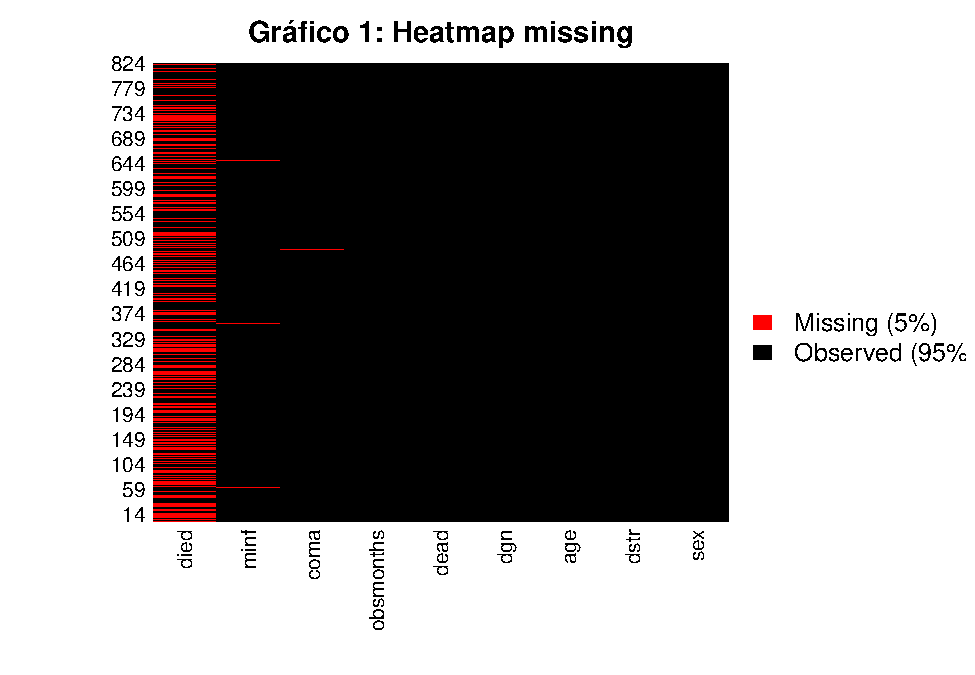
\includegraphics[width=0.6\linewidth]{Atividade_3_files/figure-latex/unnamed-chunk-1-1} \end{center}

Ao analisar o gráfico 1, a variável ``died'' apresentou quase 5\% de
valores missings, por ser uma data, não entrará na análise assim como a
variável ``dstr'', quanto as variáveis ``minf'' e ``coma'' foi optado
por remover as observações missing (10 linhas removidas, cerca de 1,21\%
dos dados).

Além disso a variável ``age'' é do tipo contínua, com a finalidade
facilitar a interpretação e a análise irei categorizar de forma binária
divididas pela mediana (71 anos), pois matém um bom balanceamento de
observações em cada categoria, como mostra a tabela abaixo

\begin{longtable}[]{@{}lr@{}}
\toprule
Age\textless{}=71 & Freq.\tabularnewline
\midrule
\endhead
FALSE & 408\tabularnewline
TRUE & 416\tabularnewline
\bottomrule
\end{longtable}

Removida as devidas variáveis e observações problemáticas podemos partir
para análise descritiva, sendo assim:

\begin{center}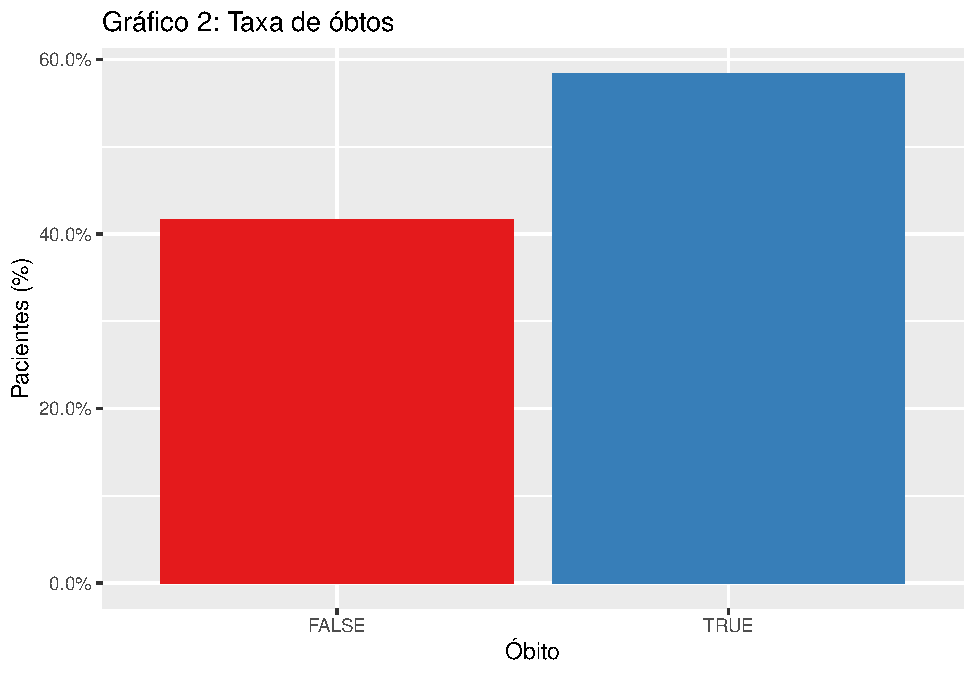
\includegraphics[width=0.6\linewidth]{Atividade_3_files/figure-latex/unnamed-chunk-3-1} \end{center}

Em que podemos notar que cerca de 60\% dos pacientes morreram.

\begin{center}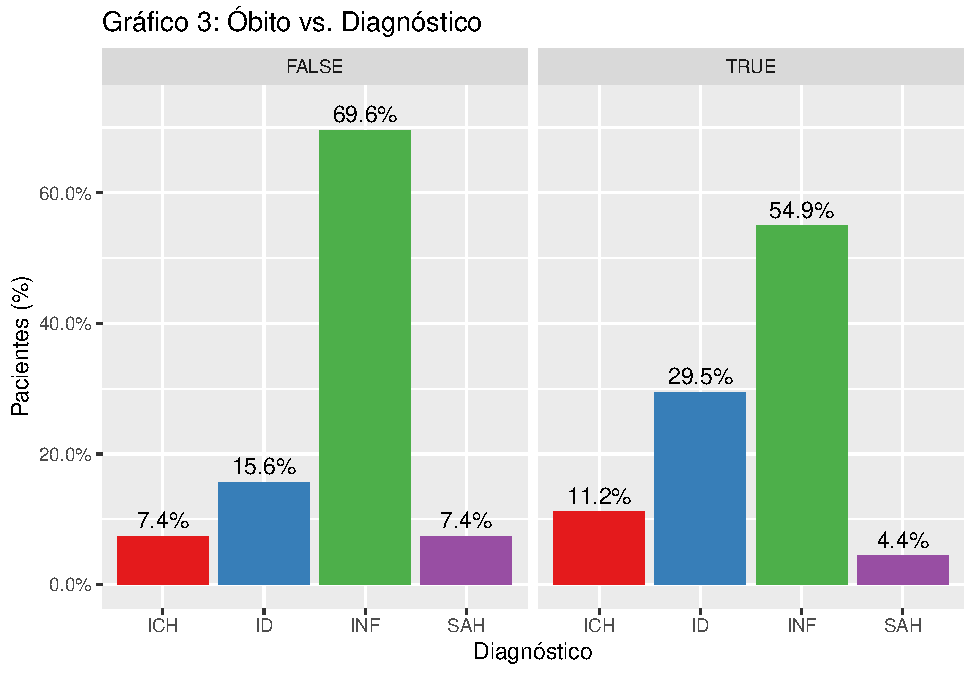
\includegraphics[width=0.7\linewidth]{Atividade_3_files/figure-latex/unnamed-chunk-4-1} \end{center}

No gráfico 3, dos pacientes que morreram cerca de 55\% tiveram o
diagnóstico ``não identificado'', seguido de 30\% com ``hemorragia
intracraniana'', enquanto isso para os pacientes que sobreviveram no
periodo do estudo, cerca de 70\% tiveram dignóstico ``não
identificado''.

\begin{center}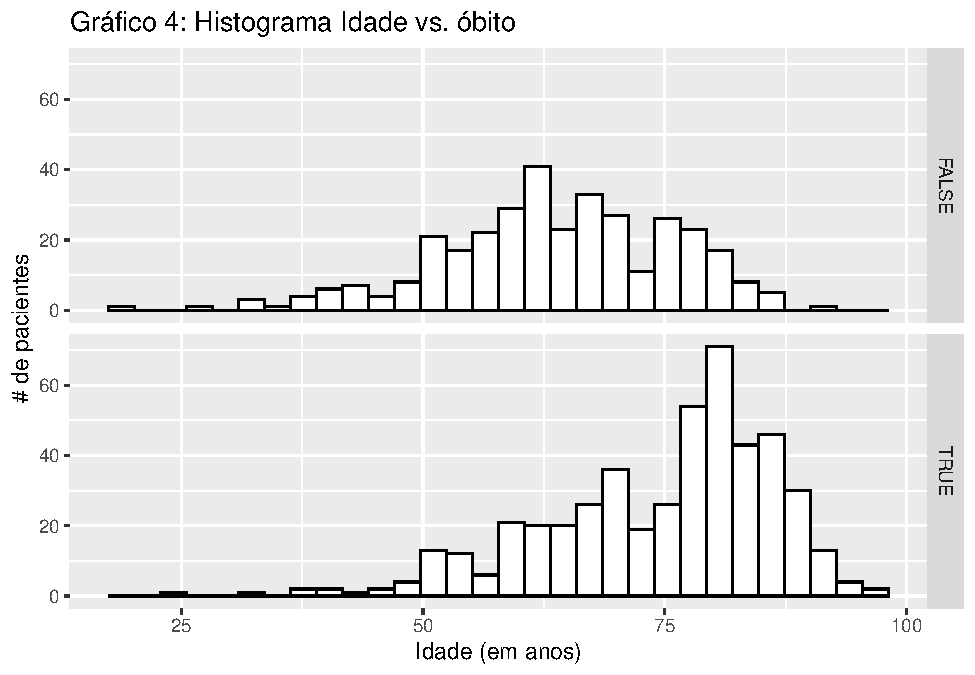
\includegraphics[width=0.7\linewidth]{Atividade_3_files/figure-latex/unnamed-chunk-5-1} \end{center}

No gráfico 4, é possível ver que a massa de pacientes que vieram a óbito
esta concentrada entre 75 e 90 anos assim como esperado, em
contrapartida os pacientes que sobreviveram durante o estudo tiveram uma
concentração de idade próximo dos 60 anos.

\begin{center}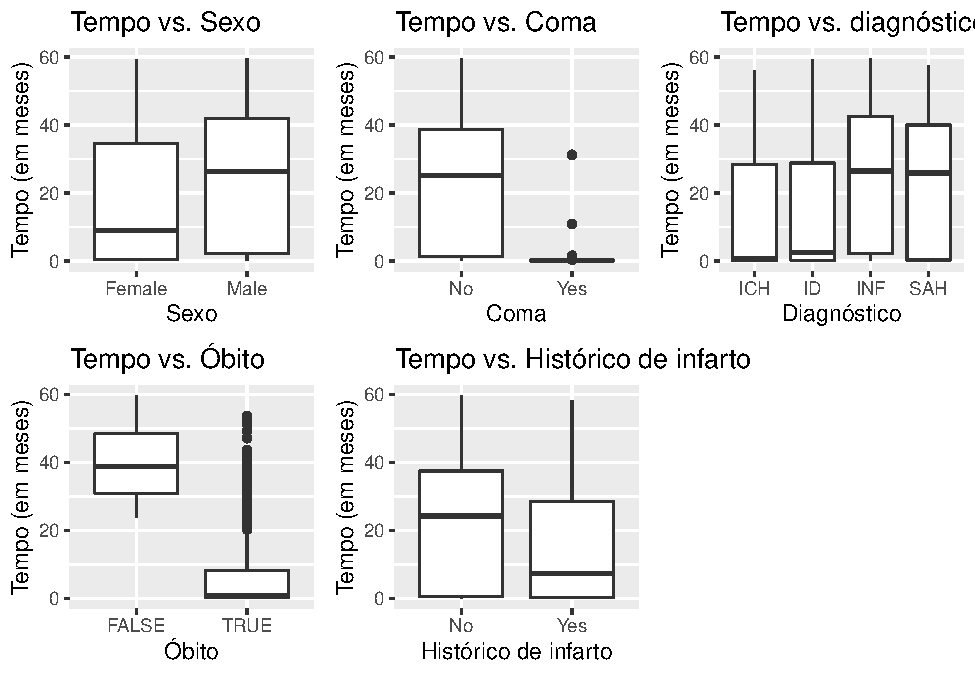
\includegraphics[width=0.8\linewidth]{Atividade_3_files/figure-latex/unnamed-chunk-6-1} \end{center}

Nos boxplots (gráficos 5 à 9) acima, temos o tempo decorrido entre
infarto e óbito ou censura contra cada covarável, e pode-se notar que os
homens tem uma mediana de tempo um pouco maior que das mulheres, também
que os pacientes que ficaram em coma tiveram o tempo muito menor contra
os que não ficaram, e assim como no gráfico 3 os pacientes
diagnosticados com hemorragia intracraniana ou não identificados tem um
tempo maior, como esperado os pacientes que vieram a óbito tiveram um
tempo menor do que os censurados e por fim os pacientes que tiveram um
histórico de infarto tiveram um tempo menor.

Avaliando os gráficos de Kaplan-Meier para cada covariável, temos:

Para a covariável sexo:

\begin{center}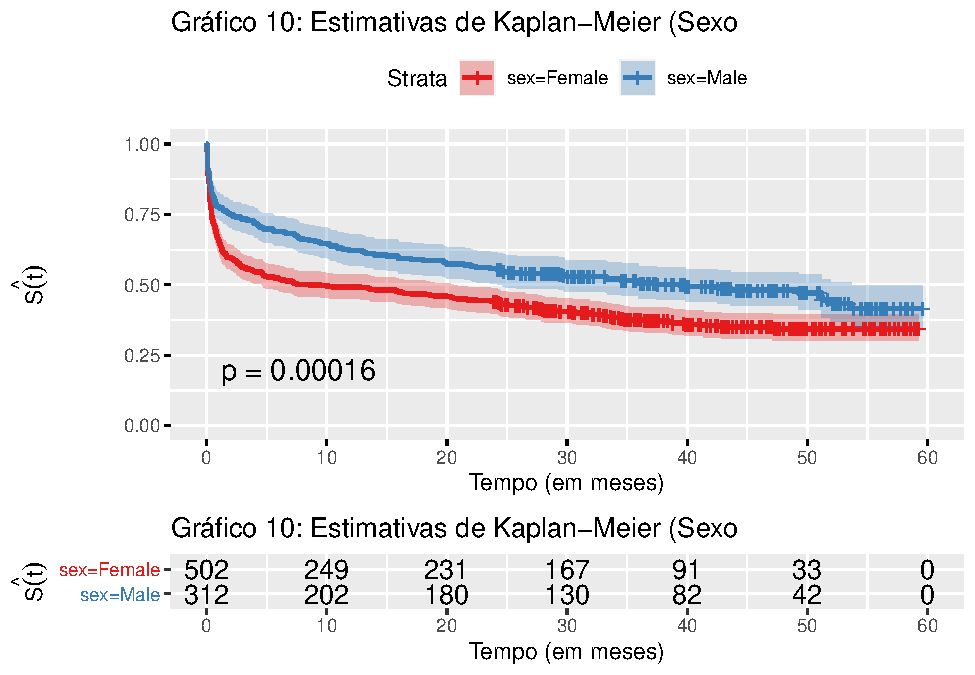
\includegraphics[width=0.8\linewidth]{Atividade_3_files/figure-latex/unnamed-chunk-7-1} \end{center}

Queremos testar a igualdade das curvas, assim:

\[ \left\{ \begin{array}{ll}
H_0: S_1(t)=S_2(t), \ \forall \ t \in \ [0,\tau] \\
H_1: S_1(t) \ne S_2(t) \ para \ algum \ t \in \ [0,\tau] \end{array} \right.\ \]

Em que \(\tau\) é o maior instante observado tal que os dois grupos
possuem pelo menos um indivíduo em risco.

Sob a hipótese nula, a estatística do teste Log-Rank é:

\[L_r=\frac{[\sum_{j=1}^{L} (d_{2j}-e_{2j})]^2}{\sum_{j=1}^{L}V_j^2}\]
Em que \(d_{2j}\) é o \(\#\) de indivíduos observados no grupo 2,
\(e_{2j}\) é o \(\#\) de indivíduos esperadados no grupo 2 e \(V_j\) é a
variância de \(d_{2j}\) que é dada por:
\[V_j=\frac{n_{1j}n_{2j}d_j(n_j-d_j)}{n_j^2(n_{1_j}-1)}\] Em que
\(n_{1j}\) e \(n_{2j}\) são o número de indivíduos nos grupo 1 e 2
respectivamente. Assim sendo, sob a hipótese nula,
\[L_r \overset{a}{\sim} \chi^2_{(1)}\]

Utilizando o teste log-rank, temos:

\begin{longtable}[]{@{}lrl@{}}
\toprule
variable & pval & method\tabularnewline
\midrule
\endhead
sex & 0.0001563 & Log-rank\tabularnewline
\bottomrule
\end{longtable}

Pelo gráfico 10 o sexo feminino aparenta possuir uma probabilidade de
sobrevivência um pouco menor do que a do sexo masculino, porém no teste
de Log-Rank e o gráfico das estimavivas de Kaplan-Meier as curvas não
são iguais a um nível de significância de 5\%.

\begin{center}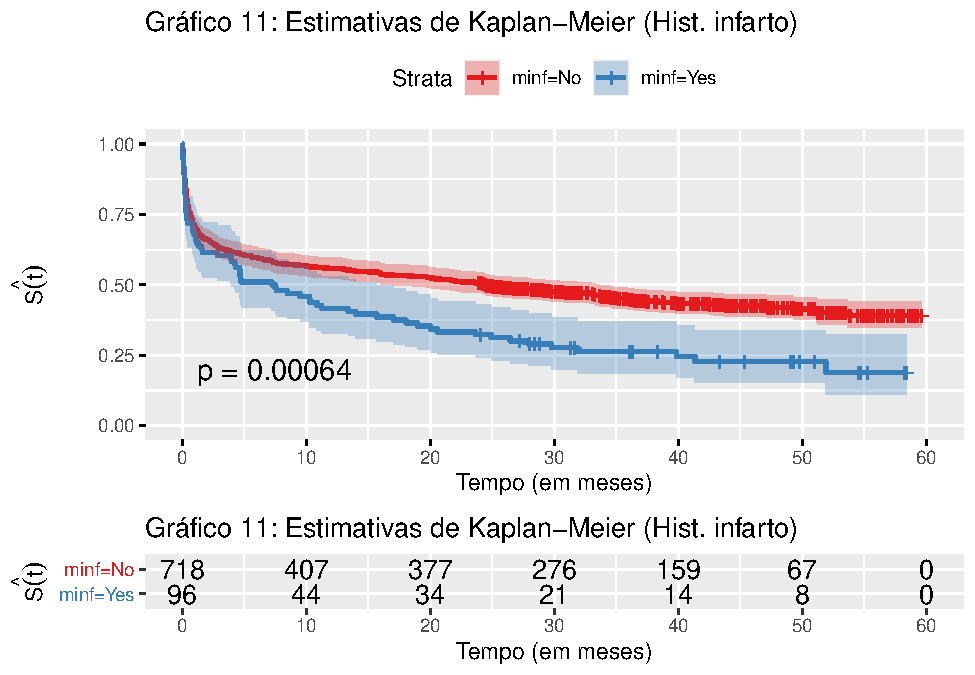
\includegraphics[width=0.75\linewidth]{Atividade_3_files/figure-latex/unnamed-chunk-9-1} \end{center}

\newpage

Utilizando o teste log-rank, temos:

\begin{longtable}[]{@{}lrl@{}}
\toprule
variable & pval & method\tabularnewline
\midrule
\endhead
minf & 0.0006447 & Log-rank\tabularnewline
\bottomrule
\end{longtable}

Pelo gráfico 11 os pacientes que tem histórico de infarto aparentam
possuir uma probabilidade de sobrevivência e um tempo de vida um pouco
menor do que a dos os pacientes que não tem histórico de infarto, porém
no teste de Log-Rank e o gráfico das estimavivas de Kaplan-Meier as
curvas não são iguais a um nível de significância de 5\%.

\begin{center}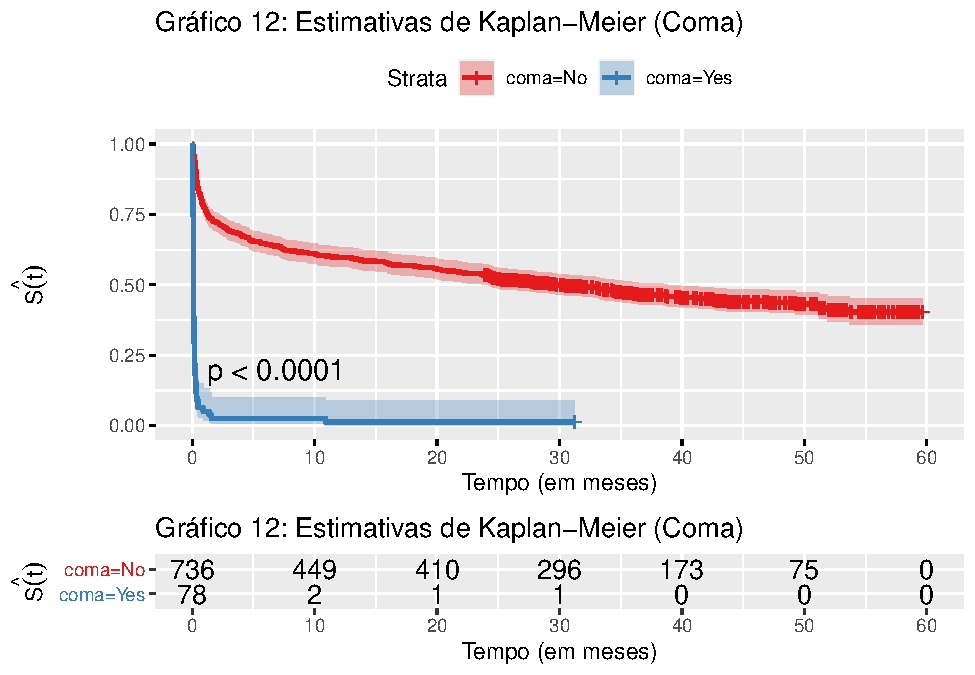
\includegraphics[width=0.8\linewidth]{Atividade_3_files/figure-latex/unnamed-chunk-11-1} \end{center}

Utilizando o teste log-rank, temos:

\begin{longtable}[]{@{}lrl@{}}
\toprule
variable & pval & method\tabularnewline
\midrule
\endhead
coma & 0 & Log-rank\tabularnewline
\bottomrule
\end{longtable}

Pelo gráfico 12 os pacientes que ficaram em coma aparentam possuir uma
probabilidade de sobrevivência e um tempo de vida muito inferior do que
a dos os pacientes que não ficaram em coma e isso se confima no teste de
Log-Rank e o gráfico das estimavivas de Kaplan-Meier as curvas não são
iguais a um nível de significância de 5\%.

\begin{center}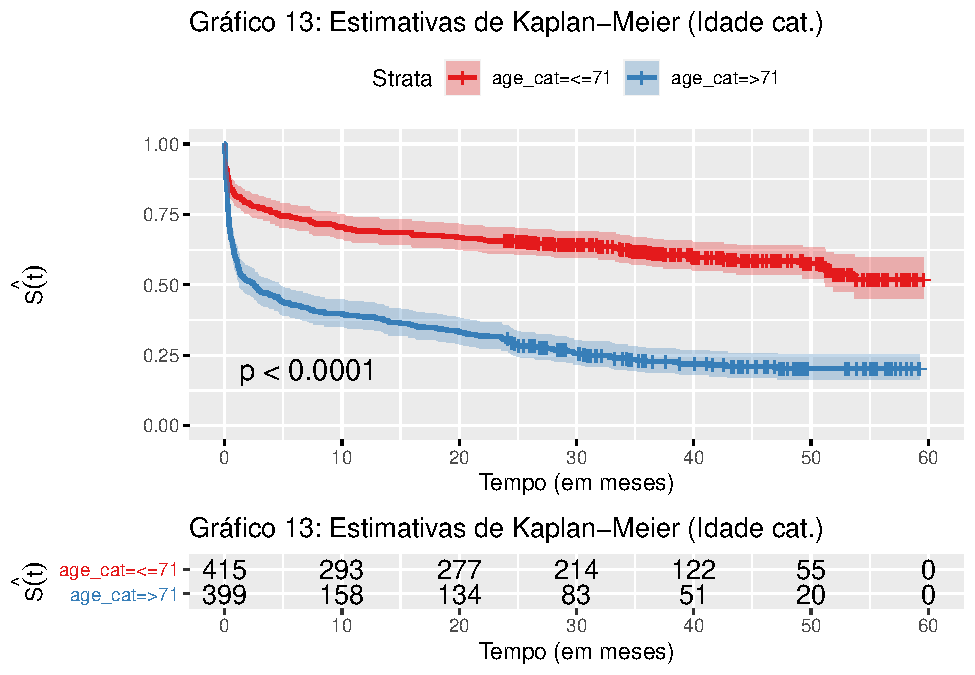
\includegraphics[width=0.8\linewidth]{Atividade_3_files/figure-latex/unnamed-chunk-13-1} \end{center}

Utilizando o teste log-rank, temos:

\begin{longtable}[]{@{}lrl@{}}
\toprule
variable & pval & method\tabularnewline
\midrule
\endhead
coma & 0 & Log-rank\tabularnewline
\bottomrule
\end{longtable}

Pelo gráfico 13 os pacientes que tem idade superior a 71 anos aparentam
possuir uma probabilidade de sobrevivência muito inferior do que a dos
os pacientes que tem menos de 71 anos e isso se confima no teste de
Log-Rank e o gráfico das estimavivas de Kaplan-Meier as curvas não são
iguais a um nível de significância de 5\%.

Para a covariável diagnóstico, por ter mais categorias, apresentou o
seguinte gráfico com as estimativas de Kaplan-Meier:

\begin{center}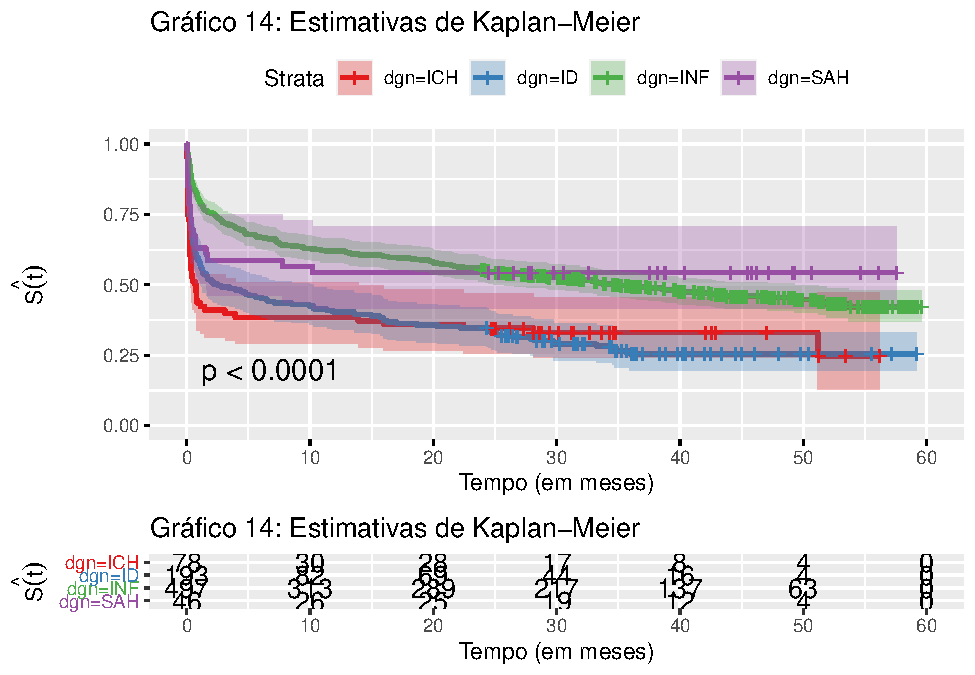
\includegraphics[width=0.8\linewidth]{Atividade_3_files/figure-latex/unnamed-chunk-15-1} \end{center}

Queremos comparar se pelo menos uma das curvas é diferente, assim
utilizando o teste log-rank generalizado, com a seguinte hipóteses,
temos:

Sob a hipótese: \[ \left\{ \begin{array}{ll}
H_0: S_1(t)=S_2(t)=S_3(t)=S_4(t), \ \forall \ t \in \ [0,\tau] \\
H_1: pelo \ menos\ uma \ funcao \ diferente  \ para \ algum \ t \in \ [0,\tau] \end{array} \right.\ \]

Utilizando o teste log-rank generalizado:

\begin{longtable}[]{@{}lrl@{}}
\toprule
variable & pval & method\tabularnewline
\midrule
\endhead
dgn & 0 & Log-rank\tabularnewline
\bottomrule
\end{longtable}

Em que segundo o teste de Log-Rank e o gráfico das estimavivas de
Kaplan-Meier pelo menos uma das curvas não são iguais a um nível de
significância de 5\%.

\begin{enumerate}
\def\labelenumi{(\alph{enumi})}
\setcounter{enumi}{1}
\tightlist
\item
  Ajuste um modelo Weibull aos dados. Apresente os resultados do modelo
  completo, com todas as covariáveis incluídas. Faça um processo de
  seleção de variáveis e apresente o resultado do modelo final obtido.
  Você precisa descrever claramente o processo de seleção das variáveis
  adotado, mas deve apresentar apenas as estimativas e resultados de
  dois modelos: modelo completo e modelo final. Você pode apresentar os
  resultados do modelo na parametrização de locação-escala.
\end{enumerate}

\newpage

\subsection{Resolução}\label{resolucao-1}

Ajustando o modelo completo com todas as variáveis:

\begin{verbatim}
## 
## Call:
## survreg(formula = Surv(obsmonths, dead) ~ sex + dgn + coma + 
##     minf + age_cat, data = data, dist = "weibull")
##               Value Std. Error      z       p
## (Intercept)  4.2803     0.3350  12.78 < 2e-16
## sexMale      0.1645     0.2122   0.78 0.43825
## dgnID        0.3139     0.3533   0.89 0.37422
## dgnINF       1.2861     0.3376   3.81 0.00014
## dgnSAH       1.1683     0.5453   2.14 0.03216
## comaYes     -4.9935     0.2767 -18.05 < 2e-16
## minfYes     -1.0284     0.2714  -3.79 0.00015
## age_cat>71  -2.2113     0.2216  -9.98 < 2e-16
## Log(scale)   0.7420     0.0389  19.07 < 2e-16
## 
## Scale= 2.1 
## 
## Weibull distribution
## Loglik(model)= -1517.2   Loglik(intercept only)= -1704.9
##  Chisq= 375.3 on 7 degrees of freedom, p= 4.7e-77 
## Number of Newton-Raphson Iterations: 5 
## n= 814
\end{verbatim}

Após o ajuste do modelo acima, nota-se que a varável sexo não é
significativa a um nível de significância de 5\%, opta-se por remove la
do modelo, alternativamente testei o método de stepwise e obtive o mesmo
resultado com apenas a remoção da variável sexo, otendo assim um modelo
com menor AIC, ajustando novamente:

\begin{verbatim}
## 
## Call:
## survreg(formula = Surv(obsmonths, dead) ~ dgn + coma + minf + 
##     age_cat, data = data, dist = "weibull")
##               Value Std. Error      z       p
## (Intercept)  4.3577     0.3207  13.59 < 2e-16
## dgnID        0.3074     0.3528   0.87 0.38349
## dgnINF       1.2945     0.3368   3.84 0.00012
## dgnSAH       1.1599     0.5448   2.13 0.03326
## comaYes     -4.9980     0.2763 -18.09 < 2e-16
## minfYes     -1.0103     0.2703  -3.74 0.00019
## age_cat>71  -2.2500     0.2163 -10.40 < 2e-16
## Log(scale)   0.7417     0.0389  19.04 < 2e-16
## 
## Scale= 2.1 
## 
## Weibull distribution
## Loglik(model)= -1517.5   Loglik(intercept only)= -1704.9
##  Chisq= 374.7 on 6 degrees of freedom, p= 7.7e-78 
## Number of Newton-Raphson Iterations: 5 
## n= 814
\end{verbatim}

\newpage

\begin{enumerate}
\def\labelenumi{(\alph{enumi})}
\setcounter{enumi}{2}
\tightlist
\item
  Interprete os parâmetros do modelo final obtido em (b).
\end{enumerate}

\subsection{Resolução}\label{resolucao-2}

Como os parâmetros que o R devolve não são usuais, deve se fazer uma
pequena tranformação para a interpretação:
\[\rho=\frac{1}{\sigma} \Rightarrow \hat{\rho}=\frac{1}{\hat{\sigma}}=\frac{1}{2.1}=0.476\]
E
\[\beta=-\frac{\gamma}{\sigma} \Rightarrow \hat\beta=-\frac{\hat\gamma}{\hat\sigma}\]
Em que \(\gamma\) são os parâmetros que o R devolve, sendo assim,
escrevendo o modelo como riscos proporcionais:
\[\widehat{\alpha(t|x)}=\hat{\rho}t^{\hat{\rho}-1}e^{x'\hat{\beta}}=0.476t^{-0.524}e^{(-2.07 -0.146x_1 -0.616x_2 -0.552x_3 +2.379x_4 +0.48x_5 + 1.071x_6)}\]
Assim comparando um indivíduo \(i\) com um \(j\), temos:
\[\frac{\widehat{\alpha(t|x_i)}}{\widehat{\alpha(t|x_j)}}=\frac{\hat{\rho}t^{\hat{\rho}-1}e^{x_i'\hat{\beta}}}{\hat{\rho}t^{\hat{\rho}-1}e^{x_j'\hat{\beta}}}=e^{(x_i-x_j)'\hat\beta}\]
Então, fixando as outras covariáveis, pode-se dizer que para a
covariável dignóstico Hemorragia intracranial=1 o risco de óbito é
\(e^{-0.146}=0.86\) vezes o risco de óbito de um indivíduo com
dignóstico Hemorragia intracranial=0.

Para a covariável dignóstico Não identificado=1 o risco de óbito é
\(e^{-0.616}=0.54\) vezes o risco de óbito de um indivíduo com
dignóstico Não identificado=0.

Para a covariável dignóstico hemorragia subaracnóide=1 o risco de óbito
é \(e^{-0.552}=0.576\) vezes o risco de óbito de um indivíduo com
dignóstico hemorragia subaracnóide=0.

Para a covariável coma=``Yes'' o risco de óbito é
\((e^{2.379}-1)*100\%=9.79 \%\) maior do que risco de óbito de um
indivíduo com coma=``No''

Para a covariável minf=``Yes'' o risco de óbito é
\((e^{0.48}-1)*100\%=0.62 \%\) maior do que risco de óbito de um
indivíduo com minf=``No''

Para a covariável age\_cat=``\textgreater{}71'' o risco de óbito é
\((e^{1.071}-1)*100\%=1.92\%\) maior do que risco de óbito de um
indivíduo com age=``\textless{}71''

\newpage

\begin{enumerate}
\def\labelenumi{(\alph{enumi})}
\setcounter{enumi}{3}
\tightlist
\item
  Faça análise de resíduos do modelo final obtido em (b).
\end{enumerate}

\subsection{Resolução}\label{resolucao-3}

Os resíduos de Cox-Snell para o modelo Weibull são obtidos a seguir:

É possível elaborar gráficos desses resíduos para a análise da escolha
do modelo. Uma opção é realizar um gráfico da função de risco acumulada
para os resíduos de Cox-Snell, utilizando os estimadores de Kaplan-Meier
(em vermelho) e Nelson\_Aalen (em azul), primeiramente para o modelo
Weibull:

\begin{center}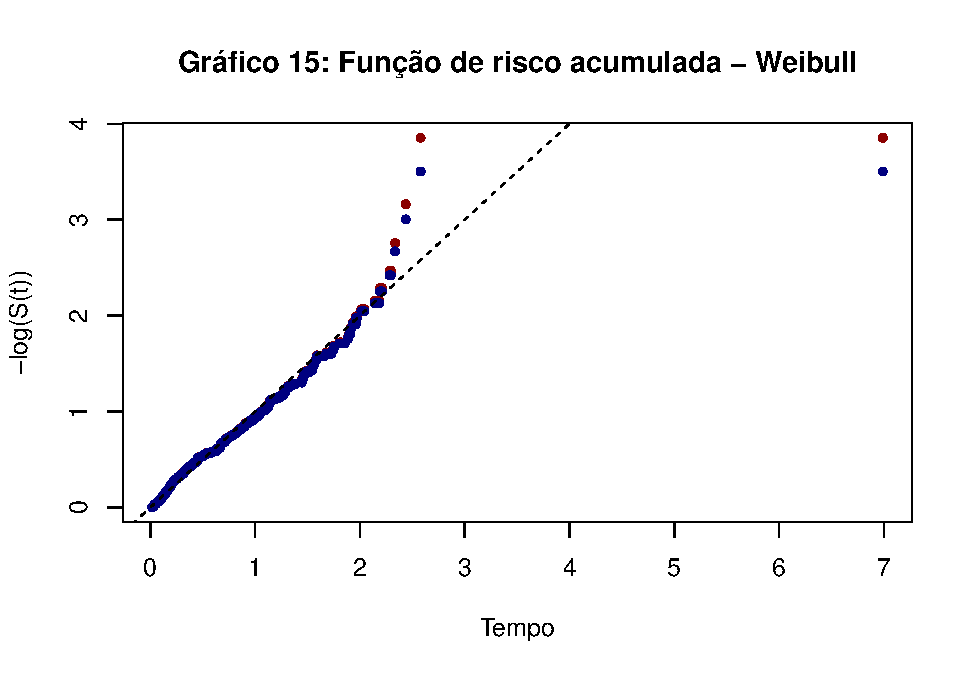
\includegraphics[width=0.8\linewidth]{Atividade_3_files/figure-latex/unnamed-chunk-19-1} \end{center}

O esperado é que os resíduos acompanhem a linha pontilhada, porém o que
vemos no gráfico 15 a partir do tempo (2,5 meses) vemos um
distanciamento da linha pontilhada

\begin{enumerate}
\def\labelenumi{(\alph{enumi})}
\setcounter{enumi}{4}
\tightlist
\item
  De forma semelhante ao item (b), ajuste um modelo log-logístico aos
  dados. Faça da mesma forma (porém utiliazndo a distribuição
  log-logística) e apresente os resultados do modelo completo e do
  modelo final.
\end{enumerate}

\newpage

\subsection{Resolução}\label{resolucao-4}

Ajustando o modelo completo com todas as variáveis:

\begin{verbatim}
## 
## Call:
## survreg(formula = Surv(obsmonths, dead) ~ sex + dgn + coma + 
##     minf + age_cat, data = data, dist = "loglogistic")
##               Value Std. Error      z       p
## (Intercept)  2.7301     0.3726   7.33 2.4e-13
## sexMale      0.3507     0.2301   1.52   0.127
## dgnID        0.8733     0.3975   2.20   0.028
## dgnINF       1.8877     0.3691   5.11 3.2e-07
## dgnSAH       1.4065     0.5850   2.40   0.016
## comaYes     -4.4449     0.3183 -13.96 < 2e-16
## minfYes     -1.0319     0.3137  -3.29   0.001
## age_cat>71  -2.3137     0.2311 -10.01 < 2e-16
## Log(scale)   0.4768     0.0388  12.29 < 2e-16
## 
## Scale= 1.61 
## 
## Log logistic distribution
## Loglik(model)= -1509.5   Loglik(intercept only)= -1685.4
##  Chisq= 351.78 on 7 degrees of freedom, p= 5.1e-72 
## Number of Newton-Raphson Iterations: 4 
## n= 814
\end{verbatim}

Após o ajuste do modelo acima, analogamente ao modelo weibull nota-se
que a varável sexo não é significativa a um nível de significância de
5\%, porém opta-se por remove la do modelo, alternativamente testei o
método de stepwise e obtive o mesmo resultado com apenas a remoção da
variável sexo, otendo assim um modelo com menor AIC, ajustando
novamente:

\begin{verbatim}
## 
## Call:
## survreg(formula = Surv(obsmonths, dead) ~ dgn + coma + minf + 
##     age_cat, data = data, dist = "loglogistic")
##               Value Std. Error      z       p
## (Intercept)  2.9072     0.3566   8.15 3.5e-16
## dgnID        0.8705     0.3988   2.18  0.0290
## dgnINF       1.9000     0.3706   5.13 3.0e-07
## dgnSAH       1.4184     0.5850   2.42  0.0153
## comaYes     -4.4465     0.3190 -13.94 < 2e-16
## minfYes     -0.9878     0.3134  -3.15  0.0016
## age_cat>71  -2.4172     0.2224 -10.87 < 2e-16
## Log(scale)   0.4790     0.0388  12.34 < 2e-16
## 
## Scale= 1.61 
## 
## Log logistic distribution
## Loglik(model)= -1510.7   Loglik(intercept only)= -1685.4
##  Chisq= 349.46 on 6 degrees of freedom, p= 2e-72 
## Number of Newton-Raphson Iterations: 4 
## n= 814
\end{verbatim}

\newpage

\begin{enumerate}
\def\labelenumi{(\alph{enumi})}
\setcounter{enumi}{5}
\tightlist
\item
  Interprete os parâmetros do modelo final obtido em (e).
\end{enumerate}

\subsection{Resolução}\label{resolucao-5}

Como os parâmetros que o R devolve não são usuais, deve se fazer uma
pequena tranformação para a interpretação:

\[\beta=-\frac{\gamma}{\sigma} \Rightarrow \hat\beta=-\frac{\hat\gamma}{\hat\sigma}\]
Com \(\hat\sigma=1.61\)

Sendo assim, escrevendo o modelo como razão de chances:
\[\frac{\widehat {S(t|x)}}{1-\widehat {S(t|x)}}=\frac{\widehat {S(t|x=0)}}{1-\widehat {S(t|x=0)}}e^{-x'\hat\beta}=t^{1/\hat\sigma}e^{-\hat\mu/\hat\sigma}e^{-x'\hat\beta}=t^{0.621}e^{-1.80}e^{(-0.54x_1 -1.18x_2 -0.881x_3 +2.762x_4 +0.613x_5 + 1.501x_6)}\]
Em que \(\hat\sigma\) é o praêmtro de escala, \(\hat\mu\) é o
intercepto, \(x'\) é a matriz de dados sem intercepto e \(\hat\beta\) é
o vetor de parâmetros. É usual interpretar os parâmetros utilizando a
razão de chances proporcionais entre um indivíduo \(i\) e outro \(j\)
com seguinte expressão:

Logo
\[\frac{\frac{\widehat {S(t|x_i)}}{1-\widehat {S(t|x_i)}}}{\frac{\widehat {S(t|x_j)}}{1-\widehat {S(t|x_j)}}}=\frac{t^{1/\hat\sigma}e^{-\hat\mu/\hat\sigma}e^{-x_i'\hat\beta}}{t^{1/\hat\sigma}e^{-\hat\mu/\hat\sigma}e^{-x_j'\hat\beta}}=e^{(x_j-x_i)'\hat\beta}\]
Então, fixando as outras covariáveis, pode-se dizer que para a
covariável dignóstico Hemorragia intracranial=1 apresentam chance de
óbito de \(e^{-0.54}=0.16\) vezes do que a de um indivíduo com
dignóstico Hemorragia intracranial=0.

Para a covariável dignóstico Não identificado=1 apresentam chance de
óbito de \(e^{-1.18}=0.37\) vezes do que a de um indivíduo com
dignóstico Não identificado=0.

Para a covariável dignóstico hemorragia subaracnóide=1 apresentam chance
de óbito é \(e^{-0.881}=0.414\) vezes do que a de um indivíduo com
dignóstico hemorragia subaracnóide=0.

Para a covariável coma=``Yes'' apresentam chance óbito é
\(e^{2.761}=15.823\) vezes do que a de um indivíduo com coma=``No''

Para a covariável minf=``Yes'' apresentam chance de óbito é
\(e^{0.635}=1.847\) vezes do que a de um indivíduo com minf=``No''

Para a covariável age\_cat=``\textgreater{}71'' apresentam chance de
óbito é \(e^{1.5}=4.49\) vezes do que a de um indivíduo com
age=``\textless{}71''

\newpage

\begin{enumerate}
\def\labelenumi{(\alph{enumi})}
\setcounter{enumi}{6}
\tightlist
\item
  Faça análise de resíduos do modelo final obtido em (e).
\end{enumerate}

\subsection{Resolução}\label{resolucao-6}

\begin{center}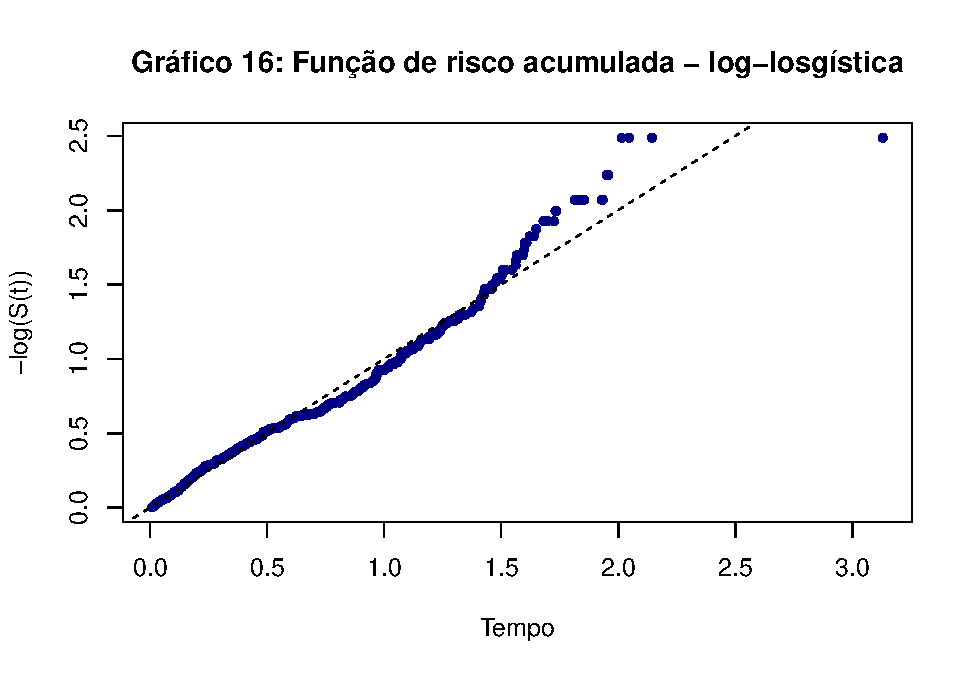
\includegraphics[width=0.8\linewidth]{Atividade_3_files/figure-latex/unnamed-chunk-22-1} \end{center}

O esperado é que os resíduos acompanhem a linha pontilhada, e o que o
gráfico 16 mostra os pontos muito próximos da linha pontilhada o que
indica um bom ajuste do modelo.

\begin{enumerate}
\def\labelenumi{(\alph{enumi})}
\setcounter{enumi}{7}
\tightlist
\item
  Compare os ajustes e os gráficos de resíduos dois modelos finais
  obtidos (com a distribuição Weibull e log-logística). Escolha um dos
  modelos para apresentar ao pesquisador como modelo final e justifique
  sua resposta.
\end{enumerate}

\subsection{Resolução}\label{resolucao-7}

Comparando os gráficos 15 e 16, quanto mais os pontos estiverem próximos
a linha pontilhada melhor é o ajuste do modelo. Logo, nota-se que pelos
gráficos do resíduos de Cox-Snell, o modelo Log-logístico possuem os
pontos mais próximos da reta pontilhada do que o modelo Weibull. Pode-se
fazer os cretérios AIC e BIC para confirmar a escolha, pela tabela
abaixo, temos:

\begin{longtable}[]{@{}lrr@{}}
\toprule
& AIC & BIC\tabularnewline
\midrule
\endhead
Weibull & 3053.038 & 3095.356\tabularnewline
Log-logistico & 3039.323 & 3081.641\tabularnewline
\bottomrule
\end{longtable}

Para o modelo log-losgístico temos um menor valor de AIC e BIC em
comparação com o modelo weibull, e associado a análise de resíduos
pode-se concluir que o modelo log-logístico esta melhor ajustado aos
dados.

\section{Anexo}\label{anexo}

\subsection{Códigos}\label{codigos}

\begin{Shaded}
\begin{Highlighting}[]
\CommentTok{# Pacotes}
\KeywordTok{library}\NormalTok{(ggplot2)}
\KeywordTok{library}\NormalTok{(survival)}
\KeywordTok{library}\NormalTok{(survminer)}
\KeywordTok{library}\NormalTok{(KMsurv)}
\KeywordTok{library}\NormalTok{(gridExtra)}
\KeywordTok{library}\NormalTok{(Amelia)}
\KeywordTok{library}\NormalTok{(RColorBrewer)}

\CommentTok{# Local de trabalho}
\KeywordTok{setwd}\NormalTok{(}\StringTok{"~/Área de Trabalho/P1 - MAE 514"}\NormalTok{)}

\CommentTok{# Leitura dos dados}
\NormalTok{data <-}\StringTok{ }\KeywordTok{read.csv}\NormalTok{(}\StringTok{"stroke_final.csv"}\NormalTok{,}\DataTypeTok{header =}\NormalTok{ T)}

\CommentTok{# Removendo a primeira coluna (desnecessária)}
\NormalTok{data}\OperatorTok{$}\NormalTok{X <-}\StringTok{ }\OtherTok{NULL}

\KeywordTok{attach}\NormalTok{(data)}

\CommentTok{# item a}
\KeywordTok{missmap}\NormalTok{(data,}\DataTypeTok{col =} \KeywordTok{c}\NormalTok{(}\StringTok{'red'}\NormalTok{,}\StringTok{'black'}\NormalTok{),}\DataTypeTok{main =} \StringTok{"Gráfico 1: Heatmap missing"}\NormalTok{)}

\NormalTok{knitr}\OperatorTok{::}\KeywordTok{kable}\NormalTok{(}\KeywordTok{table}\NormalTok{(age}\OperatorTok{<=}\DecValTok{71}\NormalTok{),}\DataTypeTok{col.names=}\KeywordTok{c}\NormalTok{(}\StringTok{'Age<=71'}\NormalTok{,}\StringTok{'Freq.'}\NormalTok{))}

\CommentTok{# categorizando variável age}

\NormalTok{data}\OperatorTok{$}\NormalTok{age_cat <-}\StringTok{ }\KeywordTok{sapply}\NormalTok{(data}\OperatorTok{$}\NormalTok{age,}
                      \ControlFlowTok{function}\NormalTok{(x)\{}
                        \ControlFlowTok{if}\NormalTok{ (x }\OperatorTok{<=}\StringTok{ }\DecValTok{71}\NormalTok{) x =}\StringTok{ '<=71'}
                        \ControlFlowTok{else}\NormalTok{ x =}\StringTok{ '>71'}
\NormalTok{                      \})}
\NormalTok{data}\OperatorTok{$}\NormalTok{age_cat <-}\StringTok{ }\KeywordTok{as.factor}\NormalTok{(data}\OperatorTok{$}\NormalTok{age_cat)}

\NormalTok{data}\OperatorTok{$}\NormalTok{died <-}\StringTok{ }\OtherTok{NULL}
\NormalTok{data}\OperatorTok{$}\NormalTok{dstr <-}\StringTok{ }\OtherTok{NULL}

\CommentTok{# removendo observações missing (7 observações)}
\NormalTok{data <-}\StringTok{ }\KeywordTok{subset}\NormalTok{(}\KeywordTok{subset}\NormalTok{(data, }\OperatorTok{!}\KeywordTok{is.na}\NormalTok{(minf)))}

\CommentTok{# removendo observações missing (3 observações)}
\NormalTok{data <-}\StringTok{ }\KeywordTok{subset}\NormalTok{(}\KeywordTok{subset}\NormalTok{(data, }\OperatorTok{!}\KeywordTok{is.na}\NormalTok{(coma)))}

\CommentTok{# Taxa de óbtos}
\KeywordTok{ggplot}\NormalTok{(data, }\KeywordTok{aes}\NormalTok{(}\DataTypeTok{x=}\NormalTok{ dead,}\DataTypeTok{fill=}\NormalTok{dead))}\OperatorTok{+}\StringTok{ }
\StringTok{          }\KeywordTok{geom_bar}\NormalTok{(}\KeywordTok{aes}\NormalTok{(}\DataTypeTok{y =}\NormalTok{ (..count..)}\OperatorTok{/}\KeywordTok{sum}\NormalTok{(..count..))) }\OperatorTok{+}\StringTok{ }
\StringTok{          }\KeywordTok{scale_y_continuous}\NormalTok{(}\DataTypeTok{labels=}\NormalTok{scales}\OperatorTok{::}\NormalTok{percent) }\OperatorTok{+}
\StringTok{  }\KeywordTok{theme}\NormalTok{(}\DataTypeTok{legend.position =} \StringTok{"none"}\NormalTok{) }\OperatorTok{+}
\StringTok{  }\KeywordTok{scale_fill_brewer}\NormalTok{(}\DataTypeTok{palette=}\StringTok{"Set1"}\NormalTok{) }\OperatorTok{+}
\StringTok{  }\KeywordTok{labs}\NormalTok{(}\DataTypeTok{y =} \StringTok{"Pacientes (%)"}\NormalTok{,}
       \DataTypeTok{x=}\StringTok{"Óbito"}\NormalTok{,}
       \DataTypeTok{title=}\StringTok{"Gráfico 2: Taxa de óbtos"}\NormalTok{)}

\CommentTok{# Óbito vs. Diagnóstico}
\KeywordTok{ggplot}\NormalTok{(data, }\KeywordTok{aes}\NormalTok{(}\DataTypeTok{x=}\NormalTok{ dgn,  }\DataTypeTok{group=}\NormalTok{dead)) }\OperatorTok{+}\StringTok{ }
\StringTok{    }\KeywordTok{geom_bar}\NormalTok{(}\KeywordTok{aes}\NormalTok{(}\DataTypeTok{y =}\NormalTok{ ..prop.., }\DataTypeTok{fill =} \KeywordTok{factor}\NormalTok{(..x..)), }\DataTypeTok{stat=}\StringTok{"count"}\NormalTok{) }\OperatorTok{+}
\StringTok{    }\KeywordTok{geom_text}\NormalTok{(}\KeywordTok{aes}\NormalTok{( }\DataTypeTok{label =}\NormalTok{ scales}\OperatorTok{::}\KeywordTok{percent}\NormalTok{(..prop..),}
                   \DataTypeTok{y=}\NormalTok{ ..prop.. ), }\DataTypeTok{stat=} \StringTok{"count"}\NormalTok{, }\DataTypeTok{vjust =} \OperatorTok{-}\NormalTok{.}\DecValTok{5}\NormalTok{) }\OperatorTok{+}
\StringTok{    }\KeywordTok{labs}\NormalTok{(}\DataTypeTok{y =} \StringTok{"Pacientes (%)"}\NormalTok{, }
         \DataTypeTok{x=}\StringTok{"Diagnóstico",}
\StringTok{         title="}\NormalTok{Gráfico }\DecValTok{3}\OperatorTok{:}\StringTok{ }\NormalTok{Óbito vs. Diagnóstico") }\OperatorTok{+}
\StringTok{    }\KeywordTok{facet_grid}\NormalTok{(}\OperatorTok{~}\NormalTok{dead) }\OperatorTok{+}
\StringTok{    }\KeywordTok{scale_fill_brewer}\NormalTok{(}\DataTypeTok{palette=}\StringTok{"Set1"}\NormalTok{) }\OperatorTok{+}
\StringTok{    }\KeywordTok{theme}\NormalTok{(}\DataTypeTok{legend.position =} \StringTok{"none"}\NormalTok{) }\OperatorTok{+}
\StringTok{    }\KeywordTok{scale_y_continuous}\NormalTok{(}\DataTypeTok{labels =}\NormalTok{ scales}\OperatorTok{::}\NormalTok{percent, }\DataTypeTok{limits =} \KeywordTok{c}\NormalTok{(}\DecValTok{0}\NormalTok{,}\FloatTok{0.73}\NormalTok{))}

\CommentTok{# Histograma Idade vs. óbito}
\KeywordTok{ggplot}\NormalTok{(data, }\KeywordTok{aes}\NormalTok{(}\DataTypeTok{x=}\NormalTok{age,  }\DataTypeTok{color=}\NormalTok{dead,}\DataTypeTok{fill=}\NormalTok{dead)) }\OperatorTok{+}\StringTok{ }
\StringTok{  }\KeywordTok{geom_histogram}\NormalTok{(}\DataTypeTok{color=}\StringTok{"black"}\NormalTok{, }\DataTypeTok{fill=}\StringTok{"white"}\NormalTok{)}\OperatorTok{+}
\StringTok{  }\KeywordTok{facet_grid}\NormalTok{(dead }\OperatorTok{~}\StringTok{ }\NormalTok{.) }\OperatorTok{+}\StringTok{ }
\StringTok{  }\KeywordTok{labs}\NormalTok{(}\DataTypeTok{x=}\StringTok{"Idade (em anos)"}\NormalTok{,}
       \DataTypeTok{y=}\StringTok{"# de pacientes"}\NormalTok{,}
       \DataTypeTok{title=}\StringTok{"Gráfico 4: Histograma Idade vs. óbito"}\NormalTok{)}

\CommentTok{# covariáveis vs. tempo de sobrev.}
\NormalTok{plot1 <-}\StringTok{ }\KeywordTok{ggplot}\NormalTok{(data, }\KeywordTok{aes}\NormalTok{(}\DataTypeTok{x=}\NormalTok{sex, }\DataTypeTok{y=}\NormalTok{obsmonths)) }\OperatorTok{+}\StringTok{ }
\StringTok{  }\KeywordTok{geom_boxplot}\NormalTok{() }\OperatorTok{+}
\StringTok{  }\KeywordTok{labs}\NormalTok{(}\DataTypeTok{y =} \StringTok{"Tempo (em meses)"}\NormalTok{, }
       \DataTypeTok{x =} \StringTok{"Sexo"}\NormalTok{,}
       \DataTypeTok{title =} \StringTok{"Tempo vs. Sexo"}\NormalTok{) }

\NormalTok{plot2 <-}\StringTok{ }\KeywordTok{ggplot}\NormalTok{(data, }\KeywordTok{aes}\NormalTok{(}\DataTypeTok{x=}\NormalTok{dgn, }\DataTypeTok{y=}\NormalTok{obsmonths)) }\OperatorTok{+}\StringTok{ }
\StringTok{  }\KeywordTok{geom_boxplot}\NormalTok{() }\OperatorTok{+}\StringTok{ }
\StringTok{  }\KeywordTok{labs}\NormalTok{(}\DataTypeTok{y =} \StringTok{"Tempo (em meses)"}\NormalTok{, }
       \DataTypeTok{x =} \StringTok{"Diagnóstico",}
\StringTok{       title = "}\NormalTok{Tempo vs. diagnóstico") }

\NormalTok{plot3 <-}\StringTok{ }\KeywordTok{ggplot}\NormalTok{(data, }\KeywordTok{aes}\NormalTok{(}\DataTypeTok{x=}\NormalTok{coma, }\DataTypeTok{y=}\NormalTok{obsmonths)) }\OperatorTok{+}\StringTok{ }
\StringTok{  }\KeywordTok{geom_boxplot}\NormalTok{() }\OperatorTok{+}\StringTok{ }
\StringTok{  }\KeywordTok{labs}\NormalTok{(}\DataTypeTok{y =} \StringTok{"Tempo (em meses)"}\NormalTok{, }
       \DataTypeTok{x =} \StringTok{"Coma"}\NormalTok{,}
       \DataTypeTok{title =} \StringTok{"Tempo vs. Coma"}\NormalTok{) }

\NormalTok{plot4 <-}\StringTok{ }\KeywordTok{ggplot}\NormalTok{(data, }\KeywordTok{aes}\NormalTok{(}\DataTypeTok{x=}\NormalTok{minf, }\DataTypeTok{y=}\NormalTok{obsmonths)) }\OperatorTok{+}\StringTok{ }
\StringTok{  }\KeywordTok{geom_boxplot}\NormalTok{() }\OperatorTok{+}\StringTok{ }
\StringTok{  }\KeywordTok{labs}\NormalTok{(}\DataTypeTok{y =} \StringTok{"Tempo (em meses)"}\NormalTok{, }
       \DataTypeTok{x =} \StringTok{"Histórico de infarto"}\NormalTok{,}
       \DataTypeTok{title =} \StringTok{"Tempo vs. Histórico de infarto"}\NormalTok{) }

\NormalTok{plot5 <-}\StringTok{ }\KeywordTok{ggplot}\NormalTok{(data, }\KeywordTok{aes}\NormalTok{(}\DataTypeTok{x=}\NormalTok{dead, }\DataTypeTok{y=}\NormalTok{obsmonths)) }\OperatorTok{+}\StringTok{ }
\StringTok{  }\KeywordTok{geom_boxplot}\NormalTok{() }\OperatorTok{+}\StringTok{ }
\StringTok{  }\KeywordTok{labs}\NormalTok{(}\DataTypeTok{y =} \StringTok{"Tempo (em meses)"}\NormalTok{, }
       \DataTypeTok{x =} \StringTok{"Óbito"}\NormalTok{,}
       \DataTypeTok{title =} \StringTok{"Tempo vs. Óbito"}\NormalTok{) }

\KeywordTok{grid.arrange}\NormalTok{(plot1, plot3, plot2,}
\NormalTok{             plot5, plot4, }\DataTypeTok{ncol=}\DecValTok{3}\NormalTok{,}\DataTypeTok{nrow=}\DecValTok{2}\NormalTok{)}

\NormalTok{ekm_sex <-}\StringTok{ }\KeywordTok{survfit}\NormalTok{(}\KeywordTok{Surv}\NormalTok{(obsmonths, dead)}\OperatorTok{~}\StringTok{ }\NormalTok{sex,}\DataTypeTok{data =}\NormalTok{ data)}

\CommentTok{# Grafico Kaplan-Meier sex}
\KeywordTok{ggsurvplot}\NormalTok{(ekm_sex, }\DataTypeTok{data =}\NormalTok{ data,}\DataTypeTok{conf.int =}\NormalTok{ T,}\DataTypeTok{palette=}\StringTok{"Set1"}\NormalTok{,}\DataTypeTok{pval =}\NormalTok{ T,}\DataTypeTok{risk.table =}\NormalTok{ T,}
           \DataTypeTok{ggtheme=}\KeywordTok{theme_gray}\NormalTok{()) }\OperatorTok{+}\StringTok{ }
\StringTok{  }\KeywordTok{labs}\NormalTok{(}\DataTypeTok{x=}\StringTok{"Tempo (em meses)"}\NormalTok{,}
       \DataTypeTok{y=}\KeywordTok{expression}\NormalTok{(}\KeywordTok{hat}\NormalTok{(}\KeywordTok{S}\NormalTok{(t))),}
       \DataTypeTok{title =} \StringTok{"Gráfico 10: Estimativas de Kaplan-Meier (Sexo"}\NormalTok{) }

\CommentTok{# log-rank sex}
\NormalTok{knitr}\OperatorTok{::}\KeywordTok{kable}\NormalTok{( }\KeywordTok{surv_pvalue}\NormalTok{(ekm_sex,data, }\DataTypeTok{method =} \KeywordTok{c}\NormalTok{(}\StringTok{"1"}\NormalTok{))[,}\DecValTok{1}\OperatorTok{:}\DecValTok{3}\NormalTok{])}

\NormalTok{ekm_minf <-}\StringTok{ }\KeywordTok{survfit}\NormalTok{(}\KeywordTok{Surv}\NormalTok{(obsmonths, dead)}\OperatorTok{~}\StringTok{ }\NormalTok{minf,}\DataTypeTok{data =}\NormalTok{ data)}

\CommentTok{# Grafico Kaplan-Meier hist inf}
\KeywordTok{ggsurvplot}\NormalTok{(ekm_minf, }\DataTypeTok{data =}\NormalTok{ data,}\DataTypeTok{conf.int =}\NormalTok{ T,}\DataTypeTok{palette=}\StringTok{"Set1"}\NormalTok{,}\DataTypeTok{pval =}\NormalTok{ T,}\DataTypeTok{risk.table =}\NormalTok{ T,}
           \DataTypeTok{ggtheme=}\KeywordTok{theme_gray}\NormalTok{()) }\OperatorTok{+}\StringTok{ }
\StringTok{  }\KeywordTok{labs}\NormalTok{(}\DataTypeTok{x=}\StringTok{"Tempo (em meses)"}\NormalTok{,}
       \DataTypeTok{y=}\KeywordTok{expression}\NormalTok{(}\KeywordTok{hat}\NormalTok{(}\KeywordTok{S}\NormalTok{(t))),}
       \DataTypeTok{title =} \StringTok{"Gráfico 11: Estimativas de Kaplan-Meier (Hist. infarto)"}\NormalTok{) }

\CommentTok{# log-rank hist inf}
\NormalTok{knitr}\OperatorTok{::}\KeywordTok{kable}\NormalTok{( }\KeywordTok{surv_pvalue}\NormalTok{(ekm_minf,data, }\DataTypeTok{method =} \KeywordTok{c}\NormalTok{(}\StringTok{"1"}\NormalTok{))[,}\DecValTok{1}\OperatorTok{:}\DecValTok{3}\NormalTok{])}

\NormalTok{ekm_coma <-}\StringTok{ }\KeywordTok{survfit}\NormalTok{(}\KeywordTok{Surv}\NormalTok{(obsmonths, dead)}\OperatorTok{~}\StringTok{ }\NormalTok{coma,}\DataTypeTok{data =}\NormalTok{ data)}

\CommentTok{# Grafico Kaplan-Meier coma}
\KeywordTok{ggsurvplot}\NormalTok{(ekm_coma, }\DataTypeTok{data =}\NormalTok{ data,}\DataTypeTok{conf.int =}\NormalTok{ T,}\DataTypeTok{palette=}\StringTok{"Set1"}\NormalTok{,}\DataTypeTok{pval =}\NormalTok{ T,}\DataTypeTok{risk.table =}\NormalTok{ T,}
           \DataTypeTok{ggtheme=}\KeywordTok{theme_gray}\NormalTok{()) }\OperatorTok{+}\StringTok{ }
\StringTok{  }\KeywordTok{labs}\NormalTok{(}\DataTypeTok{x=}\StringTok{"Tempo (em meses)"}\NormalTok{,}
       \DataTypeTok{y=}\KeywordTok{expression}\NormalTok{(}\KeywordTok{hat}\NormalTok{(}\KeywordTok{S}\NormalTok{(t))),}
       \DataTypeTok{title =} \StringTok{"Gráfico 12: Estimativas de Kaplan-Meier (Coma)"}\NormalTok{) }

\CommentTok{# log-rank coma}
\NormalTok{knitr}\OperatorTok{::}\KeywordTok{kable}\NormalTok{( }\KeywordTok{surv_pvalue}\NormalTok{(ekm_coma,data, }\DataTypeTok{method =} \KeywordTok{c}\NormalTok{(}\StringTok{"1"}\NormalTok{))[,}\DecValTok{1}\OperatorTok{:}\DecValTok{3}\NormalTok{])}

\NormalTok{ekm_age <-}\StringTok{ }\KeywordTok{survfit}\NormalTok{(}\KeywordTok{Surv}\NormalTok{(obsmonths, dead)}\OperatorTok{~}\StringTok{ }\NormalTok{age_cat,}\DataTypeTok{data =}\NormalTok{ data)}

\CommentTok{# Grafico Kaplan-Meier age cat}
\KeywordTok{ggsurvplot}\NormalTok{(ekm_age, }\DataTypeTok{data =}\NormalTok{ data,}\DataTypeTok{conf.int =}\NormalTok{ T,}\DataTypeTok{palette=}\StringTok{"Set1"}\NormalTok{,}\DataTypeTok{pval =}\NormalTok{ T,}\DataTypeTok{risk.table =}\NormalTok{ T,}
           \DataTypeTok{ggtheme=}\KeywordTok{theme_gray}\NormalTok{()) }\OperatorTok{+}\StringTok{ }
\StringTok{  }\KeywordTok{labs}\NormalTok{(}\DataTypeTok{x=}\StringTok{"Tempo (em meses)"}\NormalTok{,}
       \DataTypeTok{y=}\KeywordTok{expression}\NormalTok{(}\KeywordTok{hat}\NormalTok{(}\KeywordTok{S}\NormalTok{(t))),}
       \DataTypeTok{title =} \StringTok{"Gráfico 13: Estimativas de Kaplan-Meier (Idade cat.)"}\NormalTok{) }

\CommentTok{# log-rank age}
\NormalTok{knitr}\OperatorTok{::}\KeywordTok{kable}\NormalTok{( }\KeywordTok{surv_pvalue}\NormalTok{(ekm_age,data, }\DataTypeTok{method =} \KeywordTok{c}\NormalTok{(}\StringTok{"1"}\NormalTok{))[,}\DecValTok{1}\OperatorTok{:}\DecValTok{3}\NormalTok{])}

\NormalTok{ekm_dgn <-}\StringTok{ }\KeywordTok{survfit}\NormalTok{(}\KeywordTok{Surv}\NormalTok{(obsmonths, dead)}\OperatorTok{~}\StringTok{ }\NormalTok{dgn,}\DataTypeTok{data =}\NormalTok{ data)}

\CommentTok{# Grafico Kaplan-Meier diag}
\KeywordTok{ggsurvplot}\NormalTok{(ekm_dgn, }\DataTypeTok{data =}\NormalTok{ data,}\DataTypeTok{conf.int =}\NormalTok{ T,}\DataTypeTok{palette=}\StringTok{"Set1"}\NormalTok{,}\DataTypeTok{pval =}\NormalTok{ T,}\DataTypeTok{risk.table =}\NormalTok{ T,}
           \DataTypeTok{ggtheme=}\KeywordTok{theme_gray}\NormalTok{()) }\OperatorTok{+}\StringTok{ }
\StringTok{  }\KeywordTok{labs}\NormalTok{(}\DataTypeTok{x=}\StringTok{"Tempo (em meses)"}\NormalTok{,}
       \DataTypeTok{y=}\KeywordTok{expression}\NormalTok{(}\KeywordTok{hat}\NormalTok{(}\KeywordTok{S}\NormalTok{(t))),}
       \DataTypeTok{title =} \StringTok{"Gráfico 14: Estimativas de Kaplan-Meier"}\NormalTok{) }

\CommentTok{# log-rank diag}
\NormalTok{knitr}\OperatorTok{::}\KeywordTok{kable}\NormalTok{( }\KeywordTok{surv_pvalue}\NormalTok{(ekm_dgn,data, }\DataTypeTok{method =} \KeywordTok{c}\NormalTok{(}\StringTok{"1"}\NormalTok{))[,}\DecValTok{1}\OperatorTok{:}\DecValTok{3}\NormalTok{])}

\NormalTok{## item b}

\CommentTok{# modelo completo}
\NormalTok{mod.w <-}\StringTok{ }\KeywordTok{survreg}\NormalTok{(}\KeywordTok{Surv}\NormalTok{(obsmonths, dead)}\OperatorTok{~}\StringTok{ }\NormalTok{sex}\OperatorTok{+}\NormalTok{dgn}\OperatorTok{+}\NormalTok{coma}\OperatorTok{+}\NormalTok{minf}\OperatorTok{+}\NormalTok{age_cat, }\DataTypeTok{dist=}\StringTok{'weibull'}\NormalTok{,}
                 \DataTypeTok{data =}\NormalTok{ data)}
\KeywordTok{summary}\NormalTok{(mod.w)}

\CommentTok{#step(mod.w)}

\CommentTok{#modelo reduzido}
\NormalTok{mod.w1 <-}\StringTok{ }\KeywordTok{survreg}\NormalTok{(}\KeywordTok{Surv}\NormalTok{(obsmonths, dead)}\OperatorTok{~}\StringTok{ }\NormalTok{dgn}\OperatorTok{+}\NormalTok{coma}\OperatorTok{+}\NormalTok{minf}\OperatorTok{+}\NormalTok{age_cat, }\DataTypeTok{dist=}\StringTok{'weibull'}\NormalTok{,}
                  \DataTypeTok{data =}\NormalTok{ data)}
\KeywordTok{summary}\NormalTok{(mod.w1)}

\NormalTok{## item d}

\CommentTok{#v2 <- ifelse(data$sex=="Male",1,0)}
\NormalTok{v2 <-}\StringTok{ }\KeywordTok{ifelse}\NormalTok{(data}\OperatorTok{$}\NormalTok{dgn}\OperatorTok{==}\StringTok{"ID"}\NormalTok{,}\DecValTok{1}\NormalTok{,}\DecValTok{0}\NormalTok{)}
\NormalTok{v3 <-}\StringTok{ }\KeywordTok{ifelse}\NormalTok{(data}\OperatorTok{$}\NormalTok{dgn}\OperatorTok{==}\StringTok{"INF"}\NormalTok{,}\DecValTok{1}\NormalTok{,}\DecValTok{0}\NormalTok{)}
\NormalTok{v4 <-}\StringTok{ }\KeywordTok{ifelse}\NormalTok{(data}\OperatorTok{$}\NormalTok{dgn}\OperatorTok{==}\StringTok{"SAH"}\NormalTok{,}\DecValTok{1}\NormalTok{,}\DecValTok{0}\NormalTok{)}
\NormalTok{v5 <-}\StringTok{ }\KeywordTok{ifelse}\NormalTok{(data}\OperatorTok{$}\NormalTok{coma}\OperatorTok{==}\StringTok{"Yes"}\NormalTok{,}\DecValTok{1}\NormalTok{,}\DecValTok{0}\NormalTok{)}
\NormalTok{v6 <-}\StringTok{ }\KeywordTok{ifelse}\NormalTok{(data}\OperatorTok{$}\NormalTok{minf}\OperatorTok{==}\StringTok{"Yes"}\NormalTok{,}\DecValTok{1}\NormalTok{,}\DecValTok{0}\NormalTok{)}
\NormalTok{v7 <-}\StringTok{ }\KeywordTok{ifelse}\NormalTok{(data}\OperatorTok{$}\NormalTok{age_cat}\OperatorTok{==}\StringTok{">71"}\NormalTok{,}\DecValTok{1}\NormalTok{,}\DecValTok{0}\NormalTok{)}

\NormalTok{xb_wei <-}\StringTok{ }\NormalTok{mod.w1}\OperatorTok{$}\NormalTok{coef[}\DecValTok{1}\NormalTok{]}\OperatorTok{+}\NormalTok{mod.w1}\OperatorTok{$}\NormalTok{coef[}\DecValTok{2}\NormalTok{]}\OperatorTok{*}\NormalTok{v2}\OperatorTok{+}\NormalTok{mod.w1}\OperatorTok{$}\NormalTok{coef[}\DecValTok{3}\NormalTok{]}\OperatorTok{*}\NormalTok{v3}\OperatorTok{+}\NormalTok{mod.w1}\OperatorTok{$}\NormalTok{coef[}\DecValTok{4}\NormalTok{]}\OperatorTok{*}\NormalTok{v4}\OperatorTok{+}
\StringTok{  }\NormalTok{mod.w1}\OperatorTok{$}\NormalTok{coef[}\DecValTok{5}\NormalTok{]}\OperatorTok{*}\NormalTok{v5}\OperatorTok{+}\NormalTok{mod.w1}\OperatorTok{$}\NormalTok{coef[}\DecValTok{6}\NormalTok{]}\OperatorTok{*}\NormalTok{v6}\OperatorTok{+}\NormalTok{mod.w1}\OperatorTok{$}\NormalTok{coef[}\DecValTok{7}\NormalTok{]}\OperatorTok{*}\NormalTok{v7}

\NormalTok{coxsnell_wei<-}\StringTok{ }\NormalTok{(data}\OperatorTok{$}\NormalTok{obsmonths}\OperatorTok{^}\NormalTok{(}\DecValTok{1}\OperatorTok{/}\NormalTok{mod.w1}\OperatorTok{$}\NormalTok{scale))}\OperatorTok{*}\KeywordTok{exp}\NormalTok{(}\OperatorTok{-}\NormalTok{xb_wei}\OperatorTok{/}\NormalTok{mod.w1}\OperatorTok{$}\NormalTok{scale)}

\CommentTok{# Curva de Kaplan-Meier}
\NormalTok{KM_wei <-}\StringTok{  }\KeywordTok{survfit}\NormalTok{(}\KeywordTok{Surv}\NormalTok{(coxsnell_wei, data}\OperatorTok{$}\NormalTok{dead)}\OperatorTok{~}\DecValTok{1}\NormalTok{)}
\NormalTok{TFAcum_KM_wei <-}\StringTok{ }\OperatorTok{-}\KeywordTok{log}\NormalTok{(KM_wei}\OperatorTok{$}\NormalTok{surv)}

\CommentTok{# Estimador de Nelson_Aalen}
\NormalTok{Surv_Aa_wei <-}\StringTok{ }\KeywordTok{survfit}\NormalTok{(}\KeywordTok{coxph}\NormalTok{(}\KeywordTok{Surv}\NormalTok{(coxsnell_wei, data}\OperatorTok{$}\NormalTok{dead)}\OperatorTok{~}\DecValTok{1}\NormalTok{,}\DataTypeTok{method=}\StringTok{'breslow'}\NormalTok{))}
\NormalTok{TFAcum_Aa_wei <-}\StringTok{ }\OperatorTok{-}\KeywordTok{log}\NormalTok{(Surv_Aa_wei}\OperatorTok{$}\NormalTok{surv)}

\CommentTok{#Gráfico}
\KeywordTok{plot}\NormalTok{(KM_wei}\OperatorTok{$}\NormalTok{time,TFAcum_KM_wei, }\DataTypeTok{col=}\StringTok{"dark red"}\NormalTok{, }\DataTypeTok{pch=}\DecValTok{16}\NormalTok{,}
     \DataTypeTok{main=}\StringTok{"Gráfico 15: Função de risco acumulada - Weibull"}\NormalTok{, }\DataTypeTok{xlab=}\StringTok{"Tempo"}\NormalTok{, }\DataTypeTok{ylab=}\StringTok{"-log(S(t))"}\NormalTok{, }\DataTypeTok{cex=}\FloatTok{0.8}\NormalTok{ )}
\KeywordTok{points}\NormalTok{(Surv_Aa_wei}\OperatorTok{$}\NormalTok{time,TFAcum_Aa_wei, }\DataTypeTok{col=}\StringTok{"navy blue"}\NormalTok{, }\DataTypeTok{pch=}\DecValTok{16}\NormalTok{, }\DataTypeTok{cex=}\FloatTok{0.8}\NormalTok{)}
\KeywordTok{abline}\NormalTok{(}\DecValTok{0}\NormalTok{,}\DecValTok{1}\NormalTok{,}\DataTypeTok{lty=}\DecValTok{2}\NormalTok{)}

\NormalTok{## item e}

\CommentTok{# modelo completo}
\NormalTok{mod.ll <-}\StringTok{ }\KeywordTok{survreg}\NormalTok{(}\KeywordTok{Surv}\NormalTok{(obsmonths, dead)}\OperatorTok{~}\StringTok{ }\NormalTok{sex}\OperatorTok{+}\NormalTok{dgn}\OperatorTok{+}\NormalTok{coma}\OperatorTok{+}\NormalTok{minf}\OperatorTok{+}\NormalTok{age_cat, }\DataTypeTok{dist=}\StringTok{'loglogistic'}\NormalTok{,}\DataTypeTok{data =}\NormalTok{ data)}
\KeywordTok{summary}\NormalTok{(mod.ll)}

\CommentTok{#step(mod.w)}

\CommentTok{#modelo reduzido}
\NormalTok{mod.ll1 <-}\StringTok{ }\KeywordTok{survreg}\NormalTok{(}\KeywordTok{Surv}\NormalTok{(obsmonths, dead)}\OperatorTok{~}\StringTok{ }\NormalTok{dgn}\OperatorTok{+}\NormalTok{coma}\OperatorTok{+}\NormalTok{minf}\OperatorTok{+}\NormalTok{age_cat, }\DataTypeTok{dist=}\StringTok{'loglogistic'}\NormalTok{,}\DataTypeTok{data =}\NormalTok{ data)}
\KeywordTok{summary}\NormalTok{(mod.ll1)}

\NormalTok{## item g}

\NormalTok{xb_llog <-}\StringTok{ }\NormalTok{mod.ll1}\OperatorTok{$}\NormalTok{coef[}\DecValTok{1}\NormalTok{]}\OperatorTok{+}\NormalTok{mod.ll1}\OperatorTok{$}\NormalTok{coef[}\DecValTok{2}\NormalTok{]}\OperatorTok{*}\NormalTok{v2}\OperatorTok{+}\NormalTok{mod.ll1}\OperatorTok{$}\NormalTok{coef[}\DecValTok{3}\NormalTok{]}\OperatorTok{*}\NormalTok{v3}\OperatorTok{+}\NormalTok{mod.ll1}\OperatorTok{$}\NormalTok{coef[}\DecValTok{4}\NormalTok{]}\OperatorTok{*}\NormalTok{v4}\OperatorTok{+}\NormalTok{mod.ll1}\OperatorTok{$}\NormalTok{coef[}\DecValTok{5}\NormalTok{]}\OperatorTok{*}\NormalTok{v5}\OperatorTok{+}
\StringTok{  }\NormalTok{mod.ll1}\OperatorTok{$}\NormalTok{coef[}\DecValTok{6}\NormalTok{]}\OperatorTok{*}\NormalTok{v6}\OperatorTok{+}\NormalTok{mod.ll1}\OperatorTok{$}\NormalTok{coef[}\DecValTok{7}\NormalTok{]}\OperatorTok{*}\NormalTok{v7}

\NormalTok{coxsnell_llog <-}\StringTok{ }\KeywordTok{log}\NormalTok{(}\DecValTok{1}\OperatorTok{+}\NormalTok{(data}\OperatorTok{$}\NormalTok{obsmonths}\OperatorTok{^}\NormalTok{(}\DecValTok{1}\OperatorTok{/}\NormalTok{mod.ll1}\OperatorTok{$}\NormalTok{scale))}\OperatorTok{*}\KeywordTok{exp}\NormalTok{(}\OperatorTok{-}\NormalTok{xb_llog}\OperatorTok{/}\NormalTok{mod.ll1}\OperatorTok{$}\NormalTok{scale))}

\CommentTok{# Curva de Kaplan-Meier}
\NormalTok{KM_llog <-}\StringTok{ }\KeywordTok{survfit}\NormalTok{(}\KeywordTok{Surv}\NormalTok{(coxsnell_llog, data}\OperatorTok{$}\NormalTok{dead)}\OperatorTok{~}\DecValTok{1}\NormalTok{)}
\NormalTok{TFAcum_KM_llog <-}\StringTok{ }\OperatorTok{-}\KeywordTok{log}\NormalTok{(KM_llog}\OperatorTok{$}\NormalTok{surv)}

\CommentTok{# Estimador de Nelson_Aalen}
\NormalTok{Surv_Aa_llog <-}\StringTok{ }\KeywordTok{survfit}\NormalTok{(}\KeywordTok{coxph}\NormalTok{(}\KeywordTok{Surv}\NormalTok{(coxsnell_llog, data}\OperatorTok{$}\NormalTok{dead)}\OperatorTok{~}\DecValTok{1}\NormalTok{,}\DataTypeTok{method=}\StringTok{'breslow'}\NormalTok{))}
\NormalTok{TFAcum_Aa_llog <-}\StringTok{ }\OperatorTok{-}\KeywordTok{log}\NormalTok{(Surv_Aa_llog}\OperatorTok{$}\NormalTok{surv)}

\CommentTok{#Gráfico}
\KeywordTok{plot}\NormalTok{(KM_llog}\OperatorTok{$}\NormalTok{time,TFAcum_Aa_llog, }\DataTypeTok{col=}\StringTok{"dark red"}\NormalTok{, }\DataTypeTok{pch=}\DecValTok{16}\NormalTok{, }
     \DataTypeTok{main=}\StringTok{"Gráfico 16: Função de risco acumulada - log-losgística"}\NormalTok{, }\DataTypeTok{xlab=}\StringTok{"Tempo"}\NormalTok{, }\DataTypeTok{ylab=}\StringTok{"-log(S(t))"}\NormalTok{, }\DataTypeTok{cex=}\FloatTok{0.8}\NormalTok{ )}
\KeywordTok{points}\NormalTok{(Surv_Aa_llog}\OperatorTok{$}\NormalTok{time,TFAcum_Aa_llog, }\DataTypeTok{col=}\StringTok{"navy blue"}\NormalTok{, }\DataTypeTok{pch=}\DecValTok{16}\NormalTok{, }\DataTypeTok{cex=}\FloatTok{0.8}\NormalTok{)}
\KeywordTok{abline}\NormalTok{(}\DecValTok{0}\NormalTok{,}\DecValTok{1}\NormalTok{,}\DataTypeTok{lty=}\DecValTok{2}\NormalTok{)}

\NormalTok{## item h}

\NormalTok{AIC_llog <-}\StringTok{ }\OperatorTok{-}\DecValTok{2}\OperatorTok{*}\NormalTok{mod.ll1}\OperatorTok{$}\NormalTok{loglik[}\DecValTok{2}\NormalTok{]}\OperatorTok{+}\DecValTok{2}\OperatorTok{*}\DecValTok{9}
\NormalTok{AIC_wei <-}\StringTok{ }\OperatorTok{-}\DecValTok{2}\OperatorTok{*}\NormalTok{mod.w1}\OperatorTok{$}\NormalTok{loglik[}\DecValTok{2}\NormalTok{]}\OperatorTok{+}\DecValTok{2}\OperatorTok{*}\DecValTok{9}

\NormalTok{n <-}\StringTok{ }\KeywordTok{dim}\NormalTok{(data)[}\DecValTok{1}\NormalTok{]}

\NormalTok{BIC_wei <-}\StringTok{ }\OperatorTok{-}\DecValTok{2}\OperatorTok{*}\NormalTok{mod.w1}\OperatorTok{$}\NormalTok{loglik[}\DecValTok{2}\NormalTok{]}\OperatorTok{+}\DecValTok{9}\OperatorTok{*}\KeywordTok{log}\NormalTok{(n)}
\NormalTok{BIC_llog <-}\StringTok{ }\OperatorTok{-}\DecValTok{2}\OperatorTok{*}\NormalTok{mod.ll1}\OperatorTok{$}\NormalTok{loglik[}\DecValTok{2}\NormalTok{]}\OperatorTok{+}\DecValTok{9}\OperatorTok{*}\KeywordTok{log}\NormalTok{(n)}

\NormalTok{df <-}\StringTok{ }\KeywordTok{data.frame}\NormalTok{(}\KeywordTok{cbind}\NormalTok{(}\KeywordTok{c}\NormalTok{(AIC_wei,AIC_llog),}
\KeywordTok{c}\NormalTok{(BIC_wei,BIC_llog)),}\DataTypeTok{row.names =} \KeywordTok{c}\NormalTok{(}\StringTok{"Weibull"}\NormalTok{,}\StringTok{"Log-logistico"}\NormalTok{))}
\KeywordTok{colnames}\NormalTok{(df) <-}\StringTok{ }\KeywordTok{c}\NormalTok{(}\StringTok{'AIC'}\NormalTok{,}\StringTok{'BIC'}\NormalTok{)}

\NormalTok{knitr}\OperatorTok{::}\KeywordTok{kable}\NormalTok{(df)}
\end{Highlighting}
\end{Shaded}


\end{document}
